% ============================================================================================
% BAB III ANALISIS MASALAH
% Pembagian subbab tidak rigid dan dapat bervariasi. Bab ini minimal berisi analisis kebutuhan
% fungsional dan nonfungsional, analisis berbagai alternatif solusi yang dapat ditawarkan, dan
% metode pemilihan solusi yang diusulkan.
% ============================================================================================
\chapter{ANALISIS MASALAH}
\label{chap:analisis-masalah}

Pada bab ini dibahas analisis kondisi saat ini, analisis kebutuhan dari proses audit yang dilakukan saat ini. Selanjutnya, dilakukan analisis berbagai alternatif solusi yang dapat diusulkan untuk mengatasi permasalahan yang ada, serta metode pemilihan solusi terbaik berdasarkan kriteria yang telah ditetapkan.

\section{Analisis Kondisi Audit Energi Saat Ini}
Audit energi pada bangunan gedung saat ini umumnya masih dilaksanakan melalui proses manual yang mengikuti tahapan dasar audit energi, mulai dari penentuan ruang lingkup, pengumpulan data konsumsi energi, pengukuran lapangan, hingga perhitungan indikator kinerja dan penyusunan laporan. Literatur audit energi menunjukkan bahwa meskipun tahapan audit telah mengacu pada pedoman standar, pelaksanaannya di lapangan sering bergantung pada pencatatan manual, penggunaan \textit{spreadsheet}, dan pengolahan data yang terpisah-pisah \cite{hamdani2017audit,winarto2019audit,putra2025evaluasi}. Kondisi ini menyebabkan variasi dalam metode perhitungan, keterbatasan dokumentasi proses, serta rendahnya keterulangan hasil audit ketika dilakukan oleh auditor yang berbeda atau pada periode waktu yang berbeda.

Beberapa penelitian telah mencoba memanfaatkan perangkat lunak untuk mendukung proses audit energi, misalnya melalui sistem penilaian berbasis antarmuka grafis sederhana untuk perhitungan intensitas konsumsi energi \cite{hamdani2017audit,fitri2022sistem}. Namun, sistem-sistem tersebut umumnya masih bersifat parsial dan fokus pada fungsi tertentu, seperti pemantauan parameter listrik atau otomasi perhitungan indikator, tanpa mengintegrasikan keseluruhan alur audit energi secara \textit{end-to-end}. Keterbatasan yang masih dijumpai yaitu ketergantungan pada input manual, belum adanya mekanisme validasi dan normalisasi data terstandar, serta tidak adanya penyimpanan histori audit yang terpusat untuk mendukung analisis berkelanjutan.

Selain itu, keterbatasan instrumen pengukuran permanen dan \textit{submetering} membuat data audit sering diperoleh dari kombinasi data tagihan dan pengukuran sementara. Data yang dikumpulkan tersebut umumnya memiliki format yang tidak seragam sehingga memerlukan proses prapemrosesan tambahan sebelum dapat dianalisis. Studi audit energi pada berbagai jenis gedung menunjukkan bahwa tahapan ini menjadi salah satu sumber keterlambatan dan potensi kesalahan dalam proses audit \cite{hamdani2017audit,winarto2019audit}. Secara keseluruhan, kondisi ini menghasilkan proses audit yang memakan waktu, sulit direplikasi secara konsisten, dan kurang mendukung pemantauan kinerja energi secara berkelanjutan. Gambaran umum alur proses audit energi yang berjalan saat ini ditunjukkan pada Gambar~\ref{gambar:proses-audit-saat-ini}.

\begin{figure}[H]
    \centering
    \captionsetup{justification=centering}
        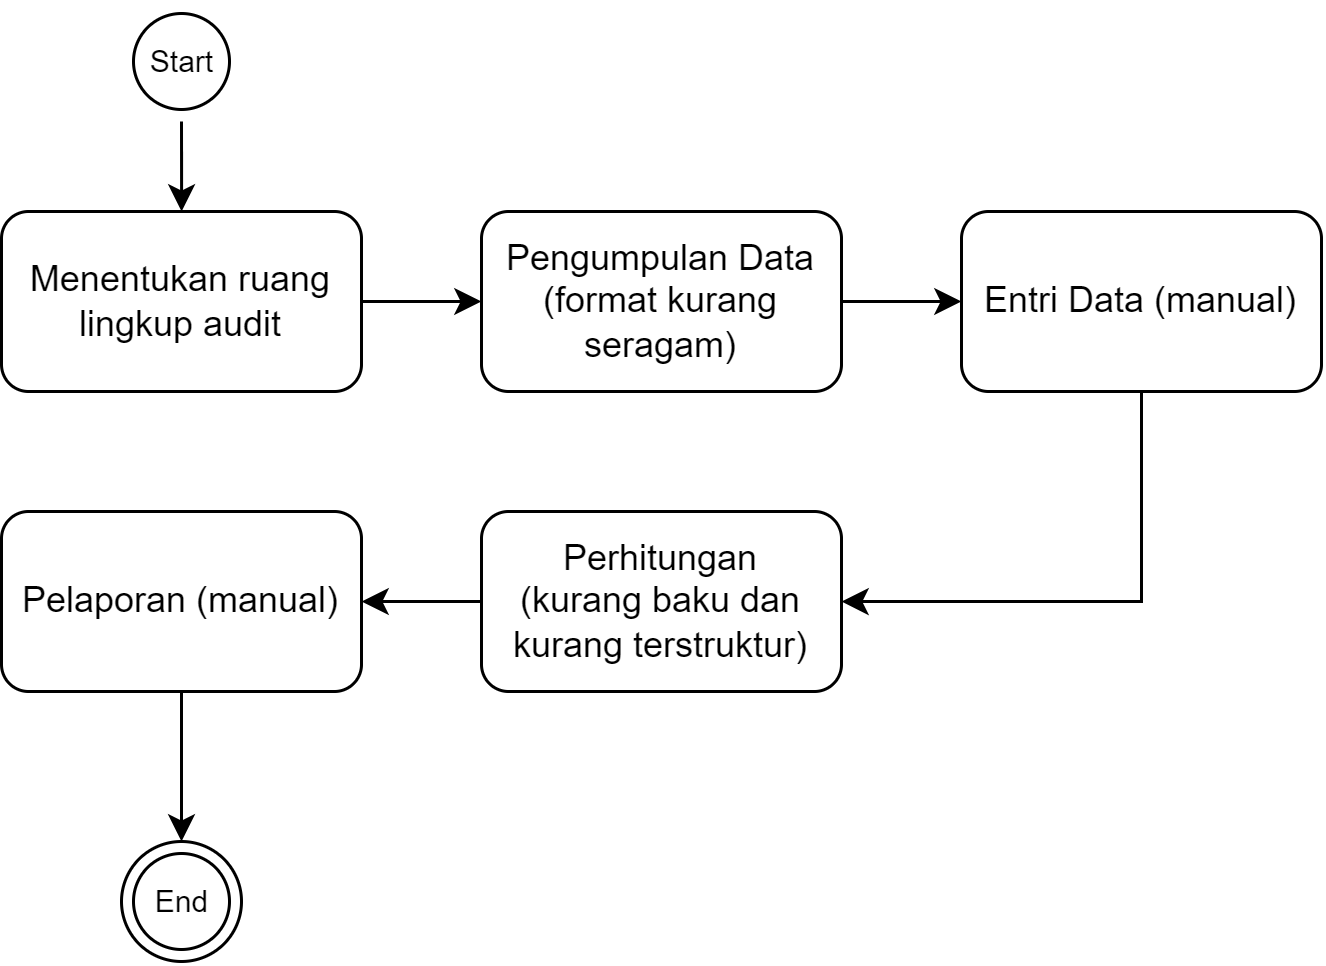
\includegraphics[width=0.7\textwidth]{image/as-is}
    \caption{Diagram Aktivitas Proses Audit Energi Saat Ini \cite{hamdani2017audit,winarto2019audit}}
    \label{gambar:proses-audit-saat-ini}
\end{figure}

Berdasarkan diagram pada Gambar~\ref{gambar:proses-audit-saat-ini}, ini merepresentasikan alur umum audit energi yang masih bersifat manual atau semimanual, sebagaimana dilaporkan dalam berbagai studi audit energi di lapangan. Proses dimulai dari penentuan ruang lingkup audit, dilanjutkan dengan pengumpulan data konsumsi energi dan hasil pengukuran lapangan yang umumnya memiliki format beragam. Data tersebut kemudian dimasukkan secara manual ke dalam \textit{spreadsheet} untuk dilakukan perhitungan indikator konsumsi energi dan penyusunan laporan hasil audit. Diagram ini ditujukan sebagai ilustrasi proses audit energi konvensional yang masih banyak dijumpai pada praktik saat ini.

Setiap tahap pada proses tersebut memiliki kendala yang cukup signifikan. Tahap pengumpulan data sering terkendala oleh keterbatasan \textit{submetering} dan ketidakteraturan format data, sehingga memerlukan waktu tambahan untuk pemeriksaan dan penyesuaian sebelum analisis dilakukan. Tahap penginputan data manual pada \textit{spreadsheet} tidak dilengkapi dengan mekanisme pemeriksaan kesalahan, sehingga meningkatkan risiko kesalahan input. Pada tahap perhitungan, penggunaan formula yang tidak terdokumentasi secara baku menyebabkan hasil audit sulit distandardisasi dan direplikasi. Proses pelaporan juga memerlukan waktu yang relatif lama karena penyusunan laporan dilakukan secara manual tanpa dukungan template atau otomatisasi.

Keterbatasan-keterbatasan tersebut berdampak langsung pada kualitas audit energi secara keseluruhan. Ketidakkonsistenan data dan metode perhitungan menurunkan keandalan hasil audit, ketiadaan basis data terpusat menghambat analisis historis dan pemantauan tren, serta lamanya proses audit menyulitkan penerapan audit energi secara berkala. Kondisi ini menegaskan perlunya suatu sistem terintegrasi yang mampu mendukung pengumpulan data, perhitungan indikator kinerja energi, dan penyusunan laporan secara lebih terstruktur, konsisten, dan efisien.

\section{Analisis Kebutuhan Perangkat Lunak Audit Energi}
Analisis kebutuhan dilakukan untuk menentukan kebutuhan sistem yang diperlukan agar proses audit energi dapat berjalan lebih efisien, akurat, dan terstruktur dibandingkan kondisi saat ini. Permasalahan pada audit manual, seperti ketidakkonsistenan data, lamanya proses perhitungan, dan ketiadaan dokumentasi historis, menunjukkan perlunya dukungan sistem yang lebih sistematis. Oleh karena itu, bagian ini membahas identifikasi masalah pengguna, kebutuhan fungsional perangkat lunak, serta kebutuhan nonfungsional yang menjadi dasar perancangan solusi pada bab selanjutnya.

\subsection{Identifikasi Masalah Pengguna Perangkat Lunak Audit Energi}
Identifikasi masalah pengguna dilakukan melalui analisis terhadap praktik audit energi yang berjalan saat ini, yang diperoleh dari studi literatur serta wawancara dengan narasumber yang memahami sistem kelistrikan bangunan dan proses audit energi serta berpengalaman di bidang energi listrik. Wawancara bertujuan untuk memperoleh gambaran mengenai parameter yang umum diperiksa dalam audit energi, proses pengumpulan dan pengolahan data energi, serta kendala yang dihadapi dalam pelaksanaannya. Berdasarkan wawancara tersebut diketahui bahwa audit energi umumnya melibatkan pengukuran parameter seperti konsumsi energi peralatan, sistem penerangan, sistem pendingin udara, serta faktor daya. Proses pengukuran sering dilakukan secara manual menggunakan instrumen lapangan seperti \textit{lux meter} dan pengukuran arus listrik, kemudian dicatat dan dianalisis menggunakan \textit{spreadsheet}. Narasumber juga menekankan bahwa kesulitan utama dalam audit energi terletak pada proses pengumpulan data, pengelolaan basis data yang kurang terstruktur, serta kebutuhan pemodelan audit yang mengacu pada standar seperti ISO 50002.

Temuan tersebut menunjukkan bahwa permasalahan dalam audit energi tidak hanya berkaitan dengan pengukuran parameter energi, tetapi juga dengan pengelolaan data, konsistensi perhitungan, serta penyajian hasil audit. Berdasarkan hasil wawancara dan kajian literatur, beberapa permasalahan utama yang dihadapi pengguna dalam proses audit energi dirumuskan dan disajikan pada Tabel~\ref{tbl:problem}.

\input table/tabelproblem.tex

Permasalahan-permasalahan pada Tabel~\ref{tbl:problem} menunjukkan bahwa proses audit energi yang dilakukan secara manual menimbulkan berbagai kendala pada tahap pengelolaan data dan analisis. Format data yang tidak seragam serta penginputan data manual menyebabkan proses normalisasi dan validasi menjadi lebih lama dan rentan terhadap kesalahan. Selain itu, metode perhitungan yang tidak terdokumentasi secara baku dapat menghasilkan perbedaan hasil audit antar periode maupun antar auditor. Ketiadaan basis data terpusat juga menyulitkan penelusuran histori audit dan analisis tren konsumsi energi jangka panjang. Permasalahan lain yang muncul adalah lamanya proses penyusunan laporan serta terbatasnya visualisasi data yang dapat membantu pengguna memahami pola konsumsi energi. Oleh karena itu, diperlukan suatu sistem yang mampu mendukung pengelolaan data audit energi secara lebih terstruktur, menyediakan perhitungan indikator yang terstandar, serta menyajikan hasil audit dalam bentuk laporan dan visualisasi yang informatif.

\subsection{Kebutuhan Fungsional Perangkat Lunak Audit Energi}
Berdasarkan hasil identifikasi masalah pengguna pada proses audit energi, dirumuskan kebutuhan fungsional yang harus dipenuhi oleh perangkat lunak audit energi yang dirancang untuk mengatasi berbagai permasalahan utama yang muncul pada audit energi konvensional, seperti ketidakkonsistenan format data, tingginya ketergantungan pada penginputan manual, perhitungan yang tidak terdokumentasi dengan baik, keterbatasan visualisasi, serta lamanya proses pelaporan. Daftar kebutuhan fungsional yang diusulkan disajikan pada Tabel~\ref{tbl:fr}, yang memuat kode kebutuhan, deskripsi fungsi sistem, serta pemetaan terhadap permasalahan pengguna yang relevan.

\input table/tabelfr.tex

Kebutuhan-kebutuhan pada Tabel~\ref{tbl:fr} menunjukkan bahwa permasalahan pada proses audit energi dapat diselesaikan oleh kebutuhan-kebutuhan tersebut. Fitur impor, input, normalisasi, dan validasi data dirancang untuk mengurangi ketidakkonsistenan format serta kesalahan penginputan data. Penyimpanan histori audit, pencatatan jejak perhitungan, dan mekanisme ekspor data. Sementara itu, \textit{dashboard} visualisasi, modul penilaian rekomendasi, dan generator laporan otomatis ditujukan untuk mempercepat analisis, meningkatkan pemahaman pengguna terhadap pola konsumsi energi, dan mempercepat tindak lanjut hasil audit. Secara keseluruhan, kebutuhan fungsional ini menjadi dasar perancangan sistem audit energi yang terintegrasi, terstandar, dan mampu mendukung proses audit secara lebih efisien dan andal dibandingkan pendekatan manual.

\subsection{Kebutuhan Nonfungsional Perangkat Lunak Audit Energi}
Selain kebutuhan fungsional, perangkat lunak audit energi juga harus memenuhi sejumlah kebutuhan nonfungsional yang dijelaskan pada Tabel~\ref{tbl:nr}. Tabel ini memuat kode kebutuhan, deskripsi singkat, serta penjelasan rinci mengenai aspek-aspek kualitas sistem yang harus dipenuhi untuk memastikan kinerja, keandalan, dan kemudahan penggunaan yang optimal.

\input table/tabelnr.tex

Kebutuhan-kebutuhan pada Tabel~\ref{tbl:nr} memastikan bahwa perangkat lunak audit energi tidak hanya memenuhi fungsi dasar, tetapi juga memiliki kualitas yang memadai. Aspek performa (\textit{performance}) menekankan pentingnya kecepatan pemrosesan data agar pengguna dapat melakukan audit dengan efisien. Keandalan (\textit{reliability}) sistem menjadi krusial untuk menjaga integritas data dan memastikan operasional yang stabil tanpa gangguan. Kemudahan penggunaan (\textit{usability}) menjadi fokus utama agar auditor, dapat mengoperasikan sistem dengan mudah dan cepat. Aspek keamanan (\textit{security}) sangat penting untuk melindungi data audit dari akses tidak sah dan menjaga kerahasiaan informasi. Skalabilitas (\textit{scalability}) memastikan bahwa sistem dapat menangani peningkatan volume data seiring waktu tanpa penurunan kinerja yang signifikan. Portabilitas (\textit{portability}) memungkinkan sistem dijalankan pada berbagai platform peramban modern tanpa memerlukan instalasi tambahan. Dengan memenuhi kebutuhan nonfungsional ini, perangkat lunak audit energi diharapkan dapat memberikan pengalaman pengguna yang baik serta menjamin kualitas dan keandalan operasional jangka panjang.

\section{Analisis Pemilihan Solusi Audit Energi}
Pada subbab ini akan dijelaskan analisis pemilihan solusi untuk menentukan solusi terbaik dari alternatif-alternatif solusi yang diusulkan. Alternatif-alternatif solusi dipilih menggunakan evaluasi berdasarkan parameter-parameter tertentu sehingga penentuan solusi yang paling sesuai dengan kebutuhan pengguna dan pengembangan perangkat lunak audit energi yang terpilih.

\subsection{Alternatif Solusi Audit Energi}
Dalam rangka mengatasi permasalahan yang telah diidentifikasi serta memenuhi kebutuhan fungsional dan nonfungsional, beberapa alternatif solusi telah dirumuskan. Tabel~\ref{tbl:altsolusi} menyajikan berbagai alternatif solusi yang dapat dipertimbangkan dengan menyatakan deskripsi singkat, kelebihan, dan kekurangan masing-masing solusi.

\input table/tabelaltsolusi.tex

\subsection{Analisis Penentuan Solusi Audit Energi}
Analisis penentuan solusi dilakukan untuk memilih alternatif solusi yang paling sesuai dengan kebutuhan dan batasan tugas akhir ini. Pemilihan solusi tidak hanya mempertimbangkan aspek teknis, tetapi juga kesesuaian dengan kebutuhan pengguna, tingkat transparansi hasil, kepatuhan terhadap standar audit energi, serta kemudahan implementasi. Untuk itu, digunakan sejumlah parameter evaluasi yang masing-masing diberikan bobot kepentingan sesuai dengan perannya dalam mendukung keberhasilan pengembangan perangkat lunak audit energi. Parameter evaluasi beserta deskripsi dan bobot kepentingannya disajikan pada Tabel~\ref{tbl:deskripsiparameteras}.

\input table/tabeldeskripsiparameteras.tex

Berdasarkan parameter dan bobot pada Tabel~\ref{tbl:deskripsiparameteras}, setiap alternatif solusi dievaluasi menggunakan pendekatan \textit{weighted scoring matrix}. Pada pendekatan ini, masing-masing solusi diberi skor terhadap setiap parameter, kemudian skor tersebut dikalikan dengan bobot parameter untuk memperoleh nilai total solusi. Pendekatan ini memungkinkan proses pemilihan solusi dilakukan secara sistematis, transparan, dan dapat dipertanggungjawabkan. Hasil evaluasi dan perbandingan nilai total setiap alternatif solusi disajikan pada Tabel~\ref{tbl:penentuansolusi}.

\input table/tabelpenentuansolusi.tex

Berdasarkan hasil analisis penentuan solusi pada Tabel~\ref{tbl:penentuansolusi}, alternatif solusi pertama, aplikasi web luring dengan sinkronisasi otomatis memperoleh nilai total tertinggi sebesar 4.55. Nilai ini lebih tinggi dibandingkan alternatif solusi kedua, sistem perhitungan dengan jejak audit terintegrasi dengan nilai 4.20, serta alternatif solusi ketiga, sistem penilaian fleksibel berbasis konfigurasi dengan nilai 3.65. Tingginya nilai solusi pertama menunjukkan bahwa pendekatan ini paling memenuhi parameter evaluasi yang ditetapkan, terutama dari sisi kelayakan teknis, kesesuaian dengan kebutuhan sistem audit energi, transparansi proses perhitungan, serta kemudahan implementasi dalam lingkup tugas akhir. Oleh karena itu, solusi aplikasi web luring dengan sinkronisasi otomatis dipilih sebagai dasar pengembangan perangkat lunak audit energi pada penelitian ini.